\begin{enumerate}[\Large\bfseries 1.]

%--------------------1.--------------------
\item  \textbf{Construcción del agregado a partir de las decisiones individuales, y cálculo del equilibrio de mercado.} Se pide:

    \begin{enumerate}

	%----------1.a.
	\item[\bfseries 1.a]  \textbf{Construcción de la curvas de demanda de mercado.} Considere dos consumidores $i$ y $h$, donde sus respectivas curvas de demanda individuales de una mercancía son:


	donde sus respectivas curvas de demanda individuales de una mercancía son:
	$$q^i = d^i(p) = 21 - p$$ $$q^h = d^h(p) = 12-2p$$ 

	\begin{enumerate}[\bfseries i)]

		%----------i)
		\item Obtenga la \textbf{curva de demanda de mercado de un bien} $Q = D(p)$ como suma horizontal de las demandas individuales $(Q = D(p) \equiv d^i(p) + d^h(p))$\\\\
	    Respuesta.-\; $$Q = D(p) \equiv d^i(p) + d^h(p) = (21 - p) + (12 - 2p) = 33-3p$$\\

		%----------ii)
		\item Dibuje las curvas de demanda individuales, y la curva de demanda de mercado una al lado de la otra horizontalmente. En los tres gráficos indique las cantidades individuales y las de mercado que se consumen a un precio $p = 4$.

	    \end{enumerate}

	    \begin{multicols}{3}
		\begin{center}
		\begin{tikzpicture}[scale=.14]
		    % abscisa y ordenada
		    \tkzInit[xmax= 23,xmin=0,ymax=23,ymin=0]
		    \tiny\tkzLabelXY[opacity=0.3,step=2, orig=false]
		    % label x, f(x)
		    \tkzDrawX[opacity= 1,label=$q^i$,right=0]
		    \tkzDrawY[opacity= 1,label=p,below = -0.2]
		    %dominio y función
		    \draw [green,domain=0:21,thick,scale=1] plot(\x,{21-\x}); 
		    \tkzText[red,above,opacity=1](10,22){\tiny $q^i = d^i(p)=21-p$}
		    \draw[blue,dashed](0,4)--(17,4)--(17,0);
		    \draw[blue](17,-1.5)node[below]{$q^i = 17$};
		    \draw[blue](-1.5,4)node[left]{$p=4$};
		\end{tikzpicture}
		\end{center}

		\begin{center}
		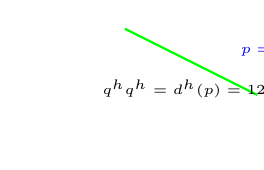
\begin{tikzpicture}[scale=.14]
		    % abscisa y ordenada
		    \tkzInit[xmax=21,xmin=0,ymax=23,ymin=0]
		    \tiny\tkzLabelXY[opacity=0.3,step=2, orig=false]
		    % label x, f(x)
		    \tkzDrawX[opacity= 1,label=$q^h$,right=0]
		    \tkzDrawY[opacity= 1,label=p,below = -0.2]
		    %dominio y función
		    \draw [green,domain=0:12,thick,scale=1] plot(\x,{6-(\x/2)}); 
		    \tkzText[red,above,opacity=1](10,22){\tiny $q^h = d^h(p) = 12-2p$}
		    \draw[blue,dashed](4,0)--(4,4)--(0,4);
		    \draw[blue](-1.5,4)node[left]{$p=4$};
		    \draw[blue](4,-1.5)node[below]{$q^i = 4$};
		\end{tikzpicture}
		\end{center}

		\begin{center}
		\begin{tikzpicture}[scale=.14]
		    % abscisa y ordenada
		    \tkzInit[xmax= 33,xmin=0,ymax=23,ymin=0]
		    \tiny\tkzLabelXY[opacity=0.3,step=2, orig=false]
		    % label x, f(x)
		    \tkzDrawX[opacity= 1,label=Q,right=0]
		    \tkzDrawY[opacity= 1,label=p,below = -0.2]
		    %dominio y función
		    \draw [green,domain=0:33,thick,scale=1] plot(\x,{11-(\x/3)}); 
		    \tkzText[red,above,opacity=1](10,22){\tiny $Q=D(p)=33-3p$}
		    \draw[blue,dashed](0,4)--(21,4)--(21,0);
		    \draw[blue](21,-3.3)node[below]{$Q = 21$};
		    \draw[blue](-1.5,4)node[left]{$p=4$};
		\end{tikzpicture}
		\end{center}
	    \end{multicols}
	    \vspace{.1cm}

	%----------1.b.
	\item[\bfseries 1.b.] \textbf{Construcción de la curvas de oferta de mercado.} Considere dos empresa, $j$ y $k$, donde sus respectivas ofertas individuales de una mercancía son:
	    $$q^j = o^j(p) = 5p-1$$ $$q^k = o^k(p) = p-2$$\\

	\begin{enumerate}[\bfseries i)]

		%----------i)
		\item Obtenga la \textbf{curva de oferta de mercado de un bien} $Q = D(p)$ como suma horizontal de las demandas individuales $(Q = O(p) \equiv o^j(p) + o^k(p))$\\\\
		    Respuesta.-\; $$Q = O(p) \equiv o^j(p) + o^k(p) = (5p-1) + (p-2) = 6p-3$$\\

		%----------ii)
		\item Dibuje las curvas de oferta individuales, y la curva de oferta de mercado una al lado de la otra horizontalmente. En los tres gráficos indique las cantidades individuales y las de mercado que se consumen a un precio $p = 4$.

	    \end{enumerate}

	    \begin{multicols}{3}
		    \begin{center}
		    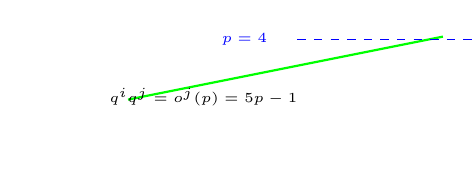
\begin{tikzpicture}[scale=.2]
			% abscisa y ordenada
			\tkzInit[xmax= 20.5,xmin=0,ymax=14,ymin=0]
			\tiny\tkzLabelXY[opacity=0.3,step=2, orig=false]
			% label x, f(x)
			\tkzDrawX[opacity= 1,label=$q^i$,right=0]
			\tkzDrawY[opacity= 1,label=p,below = -0.2]
			%dominio y función
			\draw [green,domain=0:20,thick,scale=1] plot(\x,{(\x/5)+(1/5)}); 
			\tkzText[red,above,opacity=1](10,14){\tiny $q^j = o^j(p) = 5p-1$}
			\draw[blue,dashed](0,4)--(19,4)--(19,0);
			\draw[blue](19,-2)node[below]{$q^i = 19$};
			\draw[blue](-1.5,4)node[left]{$p=4$};
		    \end{tikzpicture}
		    \end{center}

		    \begin{center}
		    \begin{tikzpicture}[scale=.2]
			% abscisa y ordenada
			\tkzInit[xmax=19,xmin=0,ymax=14,ymin=0]
			\tiny\tkzLabelXY[opacity=0.3,step=2, orig=false]
			% label x, f(x)
			\tkzDrawX[opacity= 1,label=$q^h$,right=0]
			\tkzDrawY[opacity= 1,label=p,below = -0.2]
			%dominio y función
			\draw [green,domain=0:10,thick,scale=1] plot(\x,{\x+2}); 
			\tkzText[red,above,opacity=1](10,14){\tiny $q^k = o^k(p) = p-2$}
			\draw[blue,dashed](0,4)--(2,4)--(2,0);
			\draw[blue](2,-1.5)node[below]{$q^i = 2$};
			\draw[blue](-1.5,4)node[left]{$p=4$};
		    \end{tikzpicture}
		    \end{center}

		    \begin{center}
		    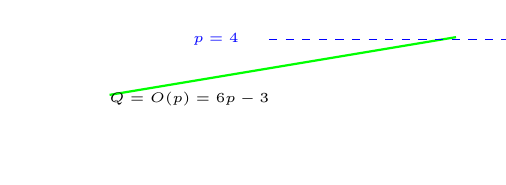
\begin{tikzpicture}[scale=.2]
			% abscisa y ordenada
			\tkzInit[xmax= 22.5,xmin=0,ymax=14,ymin=0]
			\tiny\tkzLabelXY[opacity=0.3,step=2, orig=false]
			% label x, f(x)
			\tkzDrawX[opacity= 1,label=Q,right=0]
			\tkzDrawY[opacity= 1,label=p,below = -0.2]
			%dominio y función
			\draw [green,domain=0:22,thick,scale=1] plot(\x,{(\x/6)+(1/2)}); 
			\tkzText[red,above,opacity=1](10,14){\tiny $Q=O(p)=6p-3$}
			\draw[blue,dashed](0,4)--(21,4)--(21,0);
			\draw[blue](21,-1.5)node[below]{$q^i = 21$};
			\draw[blue](-1.5,4)node[left]{$p=4$};
		    \end{tikzpicture}
		    \end{center}
	    \end{multicols}
	    \vspace{.5cm}

	%----------1.c.
	\item[\bfseries 1.c.] Obtenga el equilibrio de mercado de la mercancía.\\\\
	    Respuesta.-\; Igualando la curva de oferta y demanda tenemos el precio de equilibrio,  $$33-3p=6p-3 \; \Longrightarrow \; p=4$$
	    luego obtenemos la cantidad de equilibro reemplazando $p$ en cualquiera de las curvas dadas, $$D(p)=33-3\cdot 4 \; \Longrightarrow \; D(p)=21$$\\ 
		    \begin{center}
		    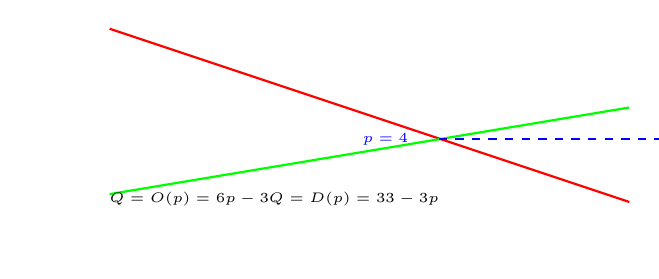
\begin{tikzpicture}[scale=.2]
			% abscisa y ordenada
			\tkzInit[xmax= 34,xmin=0,ymax=16,ymin=0]
			\tiny\tkzLabelXY[opacity=0.3,step=2, orig=false]
			% label x, f(x)
			\tkzDrawX[opacity= 1,label=Q,right=0]
			\tkzDrawY[opacity= 1,label=p,below = -0.2]
			%dominio y función
			\draw [red,domain=0:33,thick,scale=1] plot(\x,{11-(\x/3)}); 
			\draw [green,domain=0:33,thick,scale=1] plot(\x,{(\x/6)+(1/2)}); 
			\tkzText[red,above,opacity=1](14,14){\tiny $Q=O(p)=6p-3$}
			\tkzText[green,above,opacity=1](14,12){\tiny $Q=D(p)=33-3p$}
			\draw[blue,dashed](0,4)--(21,4)--(21,0);
			\draw[blue](21,-1.5)node[below]{$q = 21$};
			\draw[blue](-1.5,4)node[left]{$p=4$};
		    \end{tikzpicture}
		    \end{center}
		    \vspace{.5cm}

    \end{enumerate}

    %--------------------2.--------------------------
    \item \textbf{Bienes sustitutivos, complementarios y neutros.} En una ciudad la demanda y la oferta de un bien pueden expresarse mediante las siguientes funciones:
	$$Q^D = -2P+1,5M+6PS-4PT+300$$ $$Q^S = 2P - 8PC + 1494$$
	siendo,
	\begin{center}
	    \begin{tabular}{cl}
		$Q^D$&Cantidad demandada de bacalao al mes (en toneladas),\\
		$Q^S$&Cantidad ofrecida de bacalao al mes (en toneladas),\\
		$P$&Precio de kilo de bacalao (en Euros),\\
		$PT$&Precio de kilo de tomate frito (en Euros), cuyo valor en de $0.75$ Euros,\\
		$PS$&Precio del kilo de sardinas (en Euros), cuyo valor es de $2.5$ Euros,\\
		$PC$&Precio del litro de combustible (en Euros), cuyo valor es de $0,75$ Euros,\\
		$M$&Renta media mensual familiar (en Euros) cuyo valor es $800$ Euros.\\
	    \end{tabular}
	\end{center}
	Se pide:

	\begin{enumerate}[\bfseries a.]

	    %----------a.
	    \item Observando la función de demanda, señale las características del bien (substitutivo o complementario).\\\\
		Respuesta.-\;
		\begin{itemize}
		    \item La función de demanda nos muestra que el bacalao es un bien normal ya que puede la renta se presenta con signo positivo.
		    \item El bacalao y el tomate frito, son dos bienes complementarios. En la función de demanda podemos apreciar que en la medida en que aumente el precio del tomate estaremos menos dispuestos a comprar bacalao, o lo que es lo mismo encontraremos que el precio del tomate entra con signo negativo. 
		    \item Las sardinas y el bacalao son bienes sustitutivos, esta relación queda reflejada en el signo positivo con que aparece el precio de las sardinas en la función de demanda de bacalao. \\\\
		\end{itemize}

	    %----------b.
	    \item Obtenga las expresiones de las curvas de oferta y demanda agregadas y represéntelas gráficamente.\\\\
		Respuesta.-\; La curva de oferta agregada viene dada por:
		$$Q^S = 2P - 8\cdot 0.75 + 1494  = 2P + 1488$$
		La curva de demanda agregada viene dada por:
		$$Q^D = -2P + 1.5\cdot 800 + 6\cdot 2,5 - 4\cdot 0.75 + 300 = -2P + 1512$$
		Representamos la gráfica de la siguiente manera:

		    \begin{center}
		    \begin{tikzpicture}[scale=2]
			% abscisa y ordenada
			\tkzInit[xmax= 1510,xmin=1480,xstep=10,ymax=9,ymin=0,ystep=3]
			\tiny\tkzLabelX[opacity=0.3,step=10, orig=false]
			\tiny\tkzLabelY[opacity=0.3,step=1, orig=false]
			% label x, f(x)
			\tkzDrawX[opacity= 1,label=Q,right=0]
			\tkzDrawY[opacity= 1,label=p,below = -0.2]
			%dominio y función
			\tkzText[red,above,opacity=1](1520,8){\tiny $Q^S=2P+1488$}
			\tkzText[green,above,opacity=1](1520,7.5){\tiny $Q^D=-2P+1512$}
			\draw[green](1.44,3)--(3.12,0);
			\draw[red](0.9,0)--(2.55,3);
			\draw[blue,dashed](2,0)--(2,2)--(0,2);
		    \end{tikzpicture}
		    \end{center}
		    \vspace{.5cm}


	    %----------c.
	    \item Calcule el precio de equilibrio e indique los mecanismos por los que el mercado tendería a fijar este precio.\\\\
		Respuesta.-\; Para calcular el precio igualamos la curva de oferta y de demanda como sigue, $$2P+1488 = -2P+1542 \; \Longrightarrow \; P=6$$\\

	\end{enumerate}

    %--------------------3.
    \item \textbf{Elasticidad de la demanda de mercado.} Suponga que las personas que viajan por motivos de negocios y las que viajan de vacaciones tienen las siguientes demandas de billetes de avión entre dos ciudades:
	\begin{center}
	    \begin{tabular}{|c|r|r|}
		\hline
		\hline
		Precio&\multicolumn{2}{c|}{Cantidad de Demanda} \\ \hline
		(dólares)&Personas en viaje de negocios&Personas de vacaciones\\
		\hline
		150&2.100&1.000\\
		200&2.000&800\\
		250&1.900&600\\
		300&1.800&400\\
		\hline
		\hline
	    \end{tabular}
	\end{center}

	\begin{enumerate}[\bfseries a.]

	    %----------a.
	    \item Cuando el precio de los billetes sube de $200$ a $250$, ¿cuál es la elasticidad-precio de la demanda correspondiente a:

		\begin{enumerate}[\bfseries (i)]
		    
		    %-----(i)
		    \item las personas que viajan por motivos de negocios; y,\\\\
			Respuesta.-\; $$EP^D = \dfrac{\dfrac{Q_f-Q_i}{\dfrac{Q_i+Q_f}{2}}}{\dfrac{P_f-P_i}{\dfrac{P_i+P_f}{2}}}=\dfrac{\dfrac{1900-200}{\dfrac{2000-1900}{2}}}{\dfrac{\dfrac{250-200}{200+250}}{2}}=-0.23$$ \\

		    %-----(ii)
		    \item a las que viajan de vacaciones?\\\\
			Respuesta.-\; $$EP^D = \dfrac{\dfrac{Q_f-Q_i}{\dfrac{Q_i+Q_f}{2}}}{\dfrac{P_f-P_i}{\dfrac{P_i+P_f}{2}}}=\dfrac{\dfrac{600-800}{\dfrac{800-600}{2}}}{\dfrac{\dfrac{250-200}{200+250}}{2}}=-1.23$$\\

		\end{enumerate}

	    %----------b.
	    \item ¿Por qué tienen las personas que viajan de vacaciones una elasticidad diferente a la de las personas que viajan por motivos de negocios?\\\\
		Respuesta.-\; las personas que viajan por motivos de vacaciones tienen una elasticidad elástica ya que disminuyen la cantidad demanda donde se tiene un bien sustituto. Diferente a los que viajan por motivos de trabajo donde se tiene una elasticidad inelástica ya que es una necesidad o un bien imprescindible.\\\\

	\end{enumerate}

    %--------------------4.
    \item Estática comparativa. En una pequeña ciudad universitaria, los profesores pueden vivir en casas de su propiedad o de alquiler viviendo en alguno de los apartamentos de la residencia de la Universidad para las familias de los profesores. Centrémonos en el mercado de alquiler de apartamentos de residencias universitarias para profesores. En un curso académico existe una situación inicial de
equilibrio. Se pide (Notas. a) explique los resultados; b) se indique genéricamente a demanda o oferta: sea estricto e indique si se refiere a cantidades demandadas o a la curva de demanda, o bien a las
cantidades ofertadas o a la curva de oferta):

	\begin{enumerate}[\bfseries a.]

	    %---------a.
	    \item Defina el equilibrio en el mercado de alquiler de apartamentos de residencias universitarias para profesores.

	    %----------b.
	    \item (Estática comparativa.) Indique, ¿cómo afectará al equilibrio del mercado de alquiler para profesores después de los siguientes eventos que pueden acaecer en el siguiente curso académico?:

		\begin{enumerate}[\bfseries b.1)]

		    %-----b.1
		    \item La universidad cierra una facultad.

		    %-----b.2
		    \item La universidad cierra una de las residencias durante todo el curso para reformarla.

		    %-----b.3
		    \item Para obtener recursos, la universidad decide vender algunos de los apartamentos a los profesores que las alquilaban el curso pasado.

		\end{enumerate}
	\end{enumerate}
\end{enumerate}

